\documentclass[dvipdfmx,autodetect-engine,titlepage]{jsarticle}
\usepackage[dvipdfm]{graphicx}
\usepackage{ascmac}
\usepackage{fancybox}
\usepackage{listings}
\usepackage{plistings}
\usepackage{itembkbx}
\usepackage{amsmath}
\usepackage{svg}
\usepackage{url}
\usepackage{graphics}
\usepackage{listings,jvlisting}

\textheight=23cm
\renewcommand{\figurename}{図}
\renewcommand{\tablename}{表}
\newenvironment{code}
{\vspace{0.5zw}\VerbatimEnvironment  
\begin{screen} 
\baselineskip=1.0\normalbaselineskip
 \begin{Verbatim}}
{\end{Verbatim}
\baselineskip=\normalbaselineskip
 \end{screen}\vspace{0.5zw}} 

\title{情報理工学部 SNコース 3回\\
インシデント対応演習レポート\\}
\author{2600200443-6\\Yamashita Kyohei\\山下 恭平}
\date{Jun 5 2022}

\begin{document}

\maketitle

\section{問1:他のファイルを生成したときに何が起こるか}

暗号化された後に、再び「admin」と「AAAAABBBBB」といフォルダを生成し、
それぞれの中にテキストファイルを生成したが、しばらくするとどちらも暗号化
され、「encrypt.zip」の中に格納されていた。以下の図1,2はその様子を
示したものである。

\begin{figure}[h]
  \centering
  \begin{minipage}[b]{0.45\linewidth}
  \begin{center}
    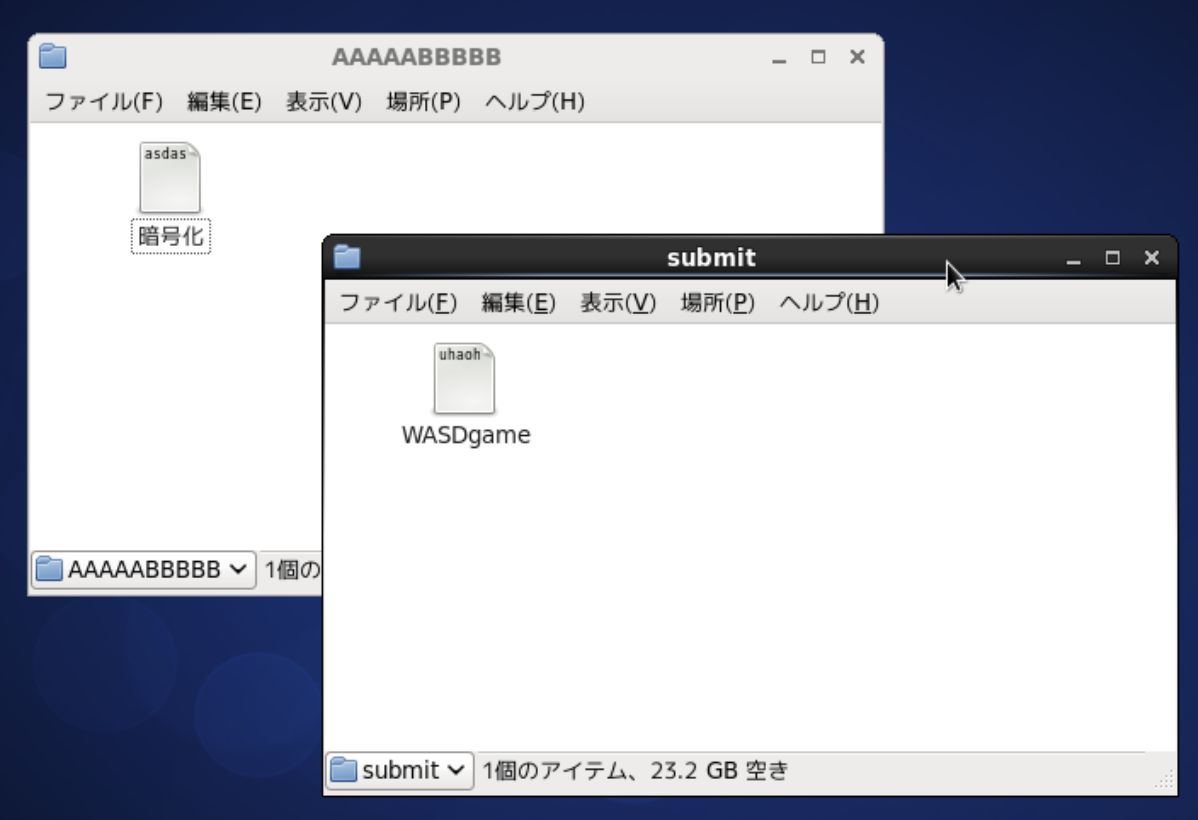
\includegraphics[keepaspectratio,scale=0.35]{pic1.png}
    \end{center}
    \caption{}
  \end{minipage}
  \begin{minipage}[b]{0.45\linewidth}
  \begin{center}
    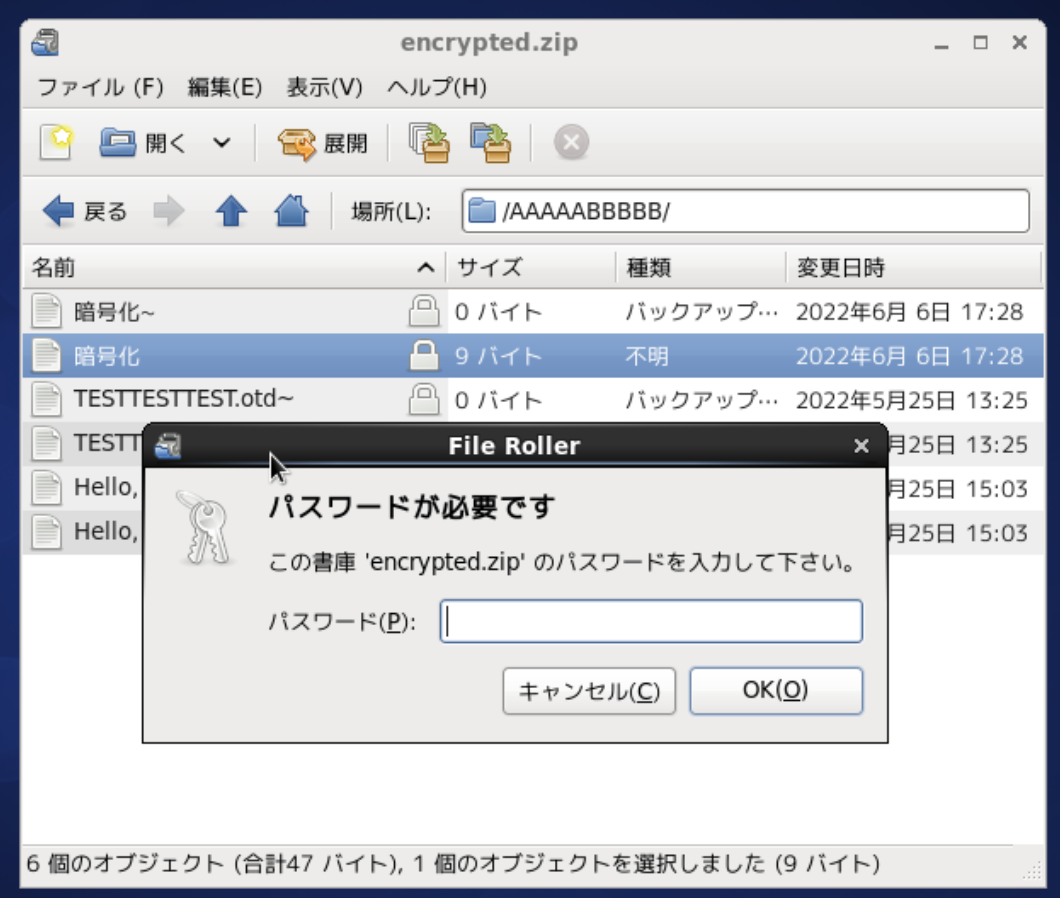
\includegraphics[keepaspectratio,scale=0.35]{pic2.png}
    \end{center}
    \caption{}
  \end{minipage}
\end{figure}

\section{問3:暗号化されたファイルを復元、またその手順}

ホームディレクトリにて、「bash\_history」ファイルの中身をcatコマンドを
用いて表示すると以下のものが得られた。

\begin{figure}[h]
  \centering
  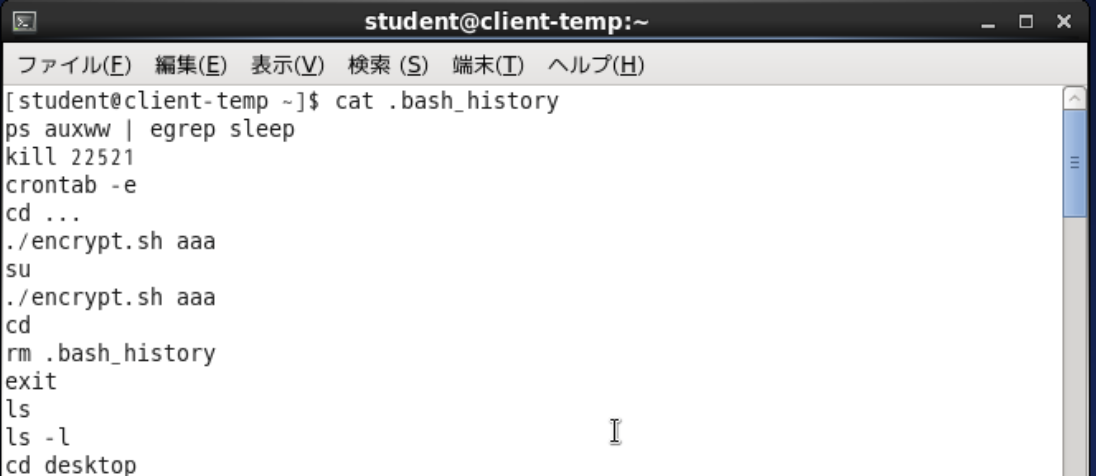
\includegraphics[scale=0.6]{pic5.png}
  \caption{}
\end{figure}

このログを見たとき、自身に身の覚えのないデジレクトリ「...」と、
覚えのないコマンド「crontab」を確認できた。ここで、「...」ディレクトリ内の
「encrypt.sh」とcrontabの中身を確認すると以下のものが得られた
\begin{figure}[h]
  \centering
  \begin{minipage}[b]{0.45\linewidth}
  \begin{center}
    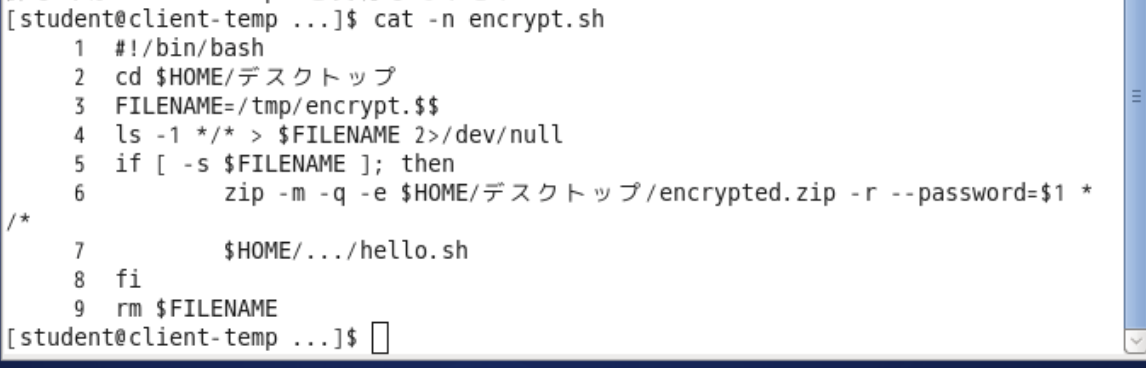
\includegraphics[keepaspectratio,scale=0.35]{pic6.png}
    \end{center}
    \caption{encrypt.sh}
  \end{minipage}
  \begin{minipage}[b]{0.45\linewidth}
  \begin{center}
    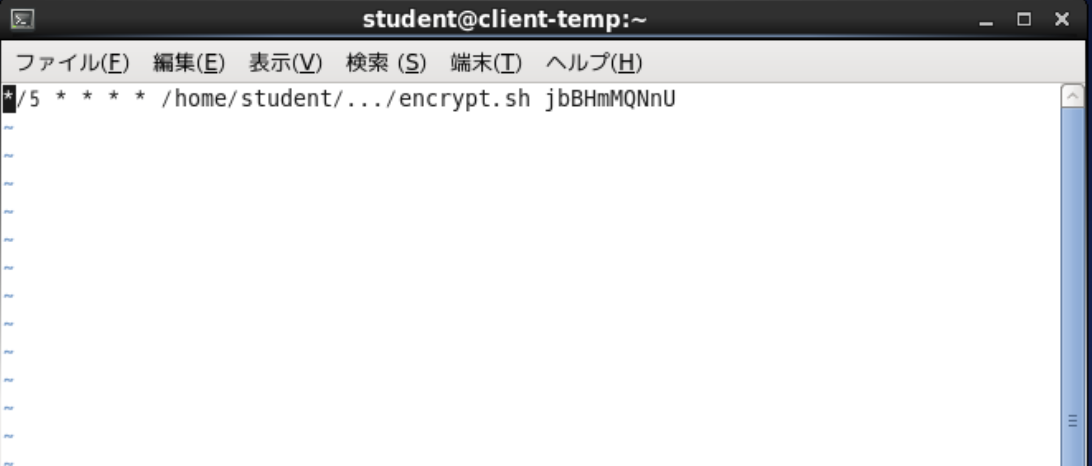
\includegraphics[keepaspectratio,scale=0.35]{pic7.png}
    \end{center}
    \caption{crontab}
  \end{minipage}
\end{figure}

 crontabの内容から、5分おきに「encrypt.sh」が実行されていることがわかる。
 また、encrypt.shの6行目より、圧縮時のパスワードはコマンドライン引数の
 1番目から取得していることがわかるので、crontabに記載されている文字列
 「jbBHmMQNnU」はパスワードであるとわかる。


\section{問2:攻撃者のメッセージに含まれる番号の意味}

受付番号は班のメンバー全員バラバラであった、また、受付番号はファイルが暗号化
されるたびに新しいものへと更新されていることがわかった。

\begin{figure}[h]
  \centering
  \begin{minipage}[b]{0.45\linewidth}
  \begin{center}
    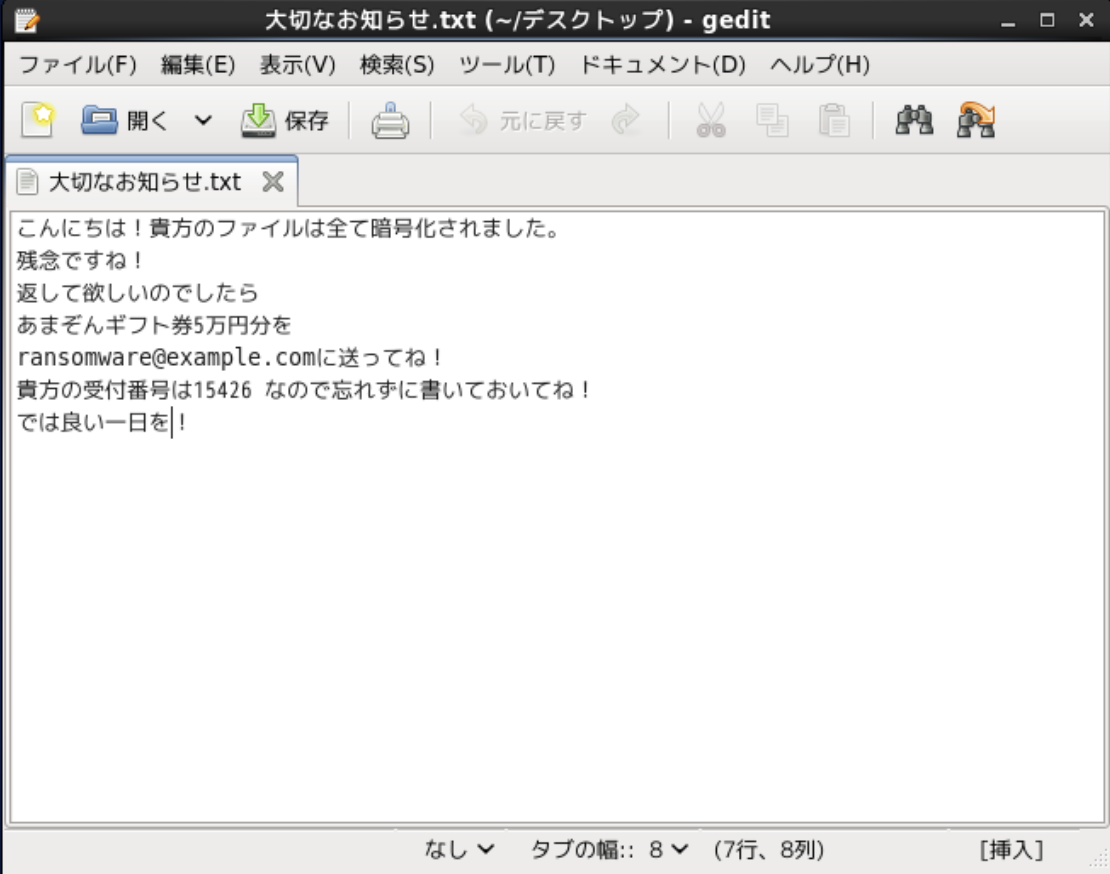
\includegraphics[keepaspectratio,scale=0.35]{pic3.png}
    \end{center}
    \caption{}
  \end{minipage}
  \begin{minipage}[b]{0.45\linewidth}
  \begin{center}
    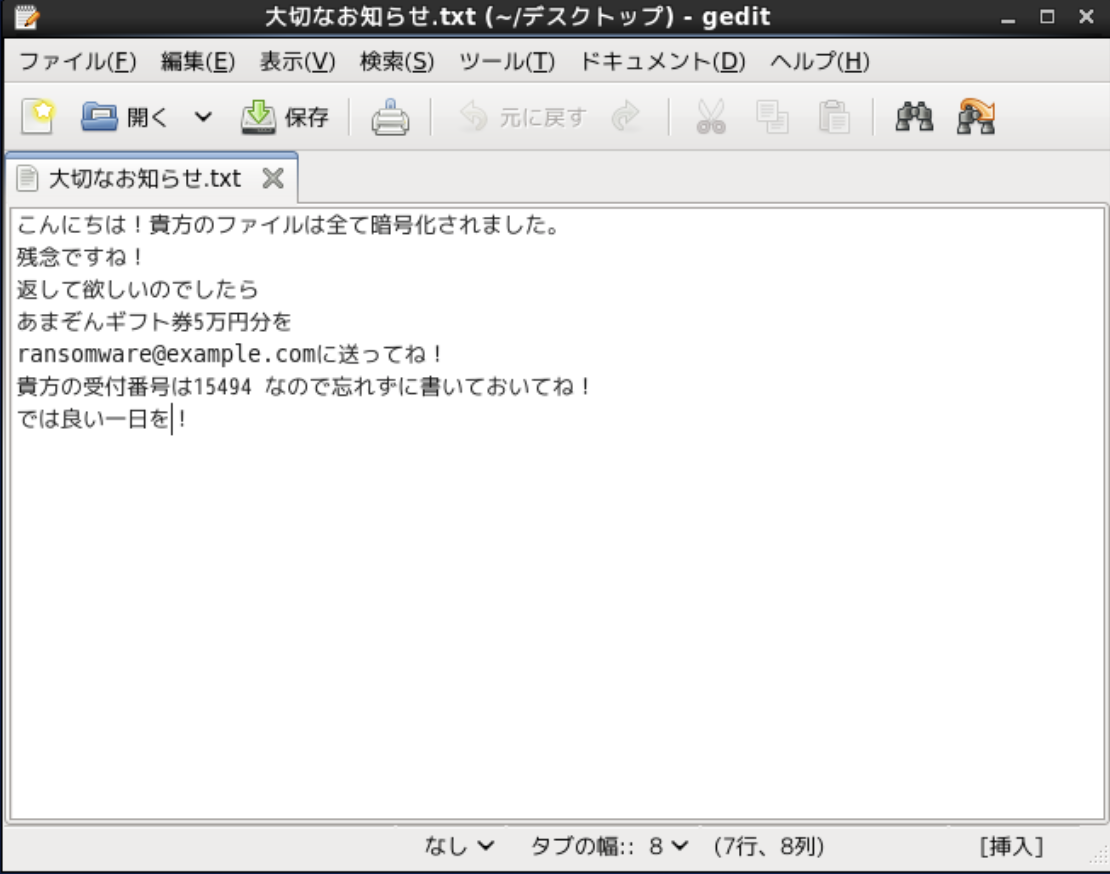
\includegraphics[keepaspectratio,scale=0.35]{pic4.png}
    \end{center}
    \caption{}
  \end{minipage}
\end{figure}

図4,encrypt.shの7行目より、「hello.sh」が呼び出されていることがわかるので
、hello.shの中身を確認すると以下のものが得られた。

\begin{figure}[h]
  \centering
  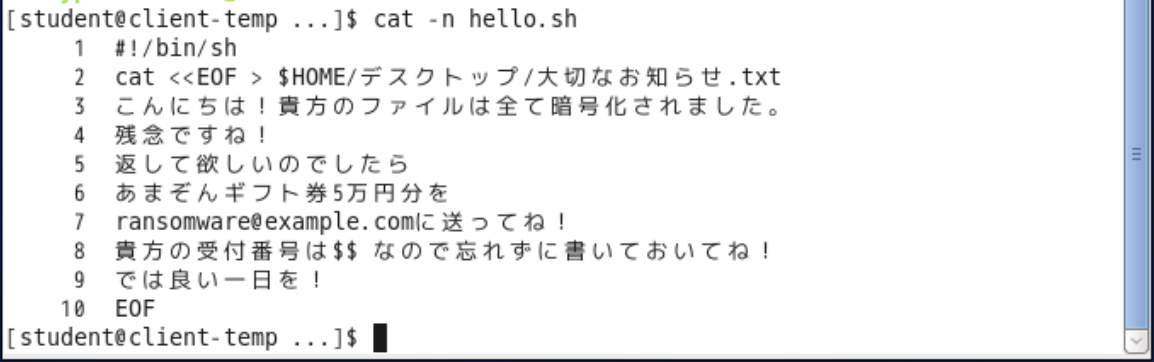
\includegraphics[scale=0.7]{pic8.png}
  \caption{hello.sh}
\end{figure}

受付番号と対応するのは8行目の「\$\$」の部分であることから、
受付番号は、hello.shが呼び出された時のプロセスIDであることが
わかる。

\section{問4:攻撃に使われたプログラムの場所}

ホームディレクトリないの「bash\_profile」を確認すると、起動後に
「fire\_crontab.sh」を呼び出していることが確認できた。「fire\_crontab.sh」
の中身を確認すると、呼び出し後600秒待機し、crontabにencrypt.shを5分に
一度起動するように書き込んでいるのが確認できる。

\begin{figure}[h]
  \centering
  \begin{minipage}[b]{0.45\linewidth}
  \begin{center}
    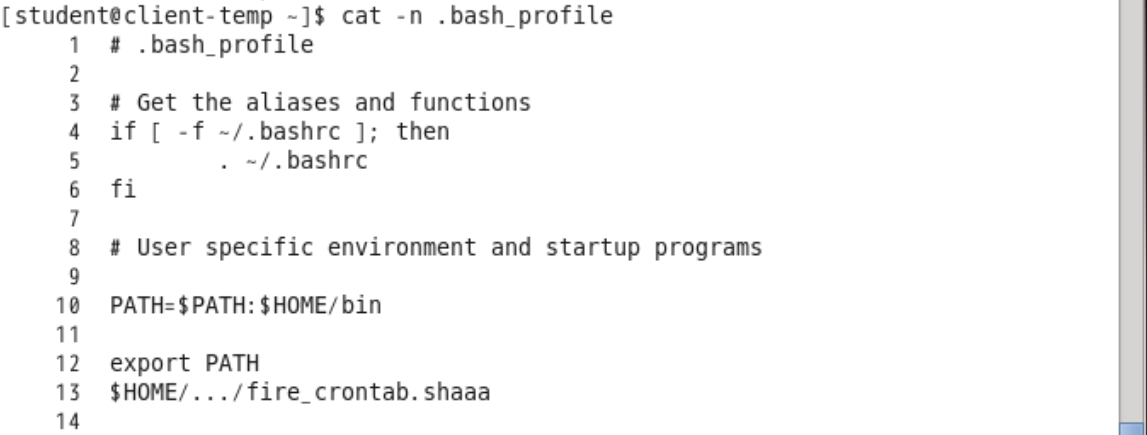
\includegraphics[keepaspectratio,scale=0.35]{pic9.png}
    \end{center}
    \caption{bash\_profile}
  \end{minipage}
  \begin{minipage}[b]{0.45\linewidth}
  \begin{center}
    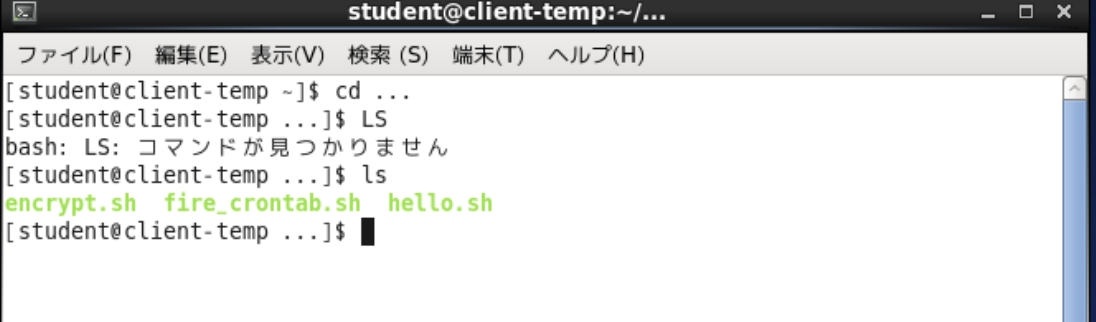
\includegraphics[keepaspectratio,scale=0.35]{pic10.png}
    \end{center}
    \caption{...}
  \end{minipage}
\end{figure}

よって、攻撃に使用されたファイル「encrypt.sh」,「hello.sh」,「fire\_crontab.sh」は
全てディレクトリ「...」に格納されている。

\begin{figure}[h]
  \centering
  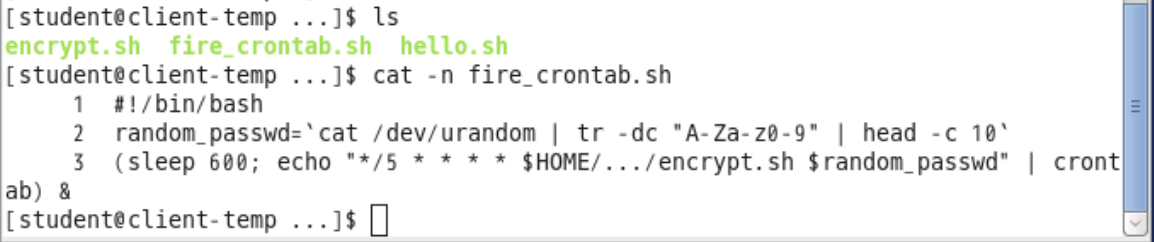
\includegraphics[scale=0.6]{pic11.png}
  \caption{fire\_crontab.sh}
\end{figure}


\section{問5:攻撃の一連の手順の予想}
攻撃者はパスワードのかかっていないアカウント「student1」にアクセスし、
攻撃の準備を整えたと考えられる。ログイン後なぜユーザ「student」へアクセスし
、攻撃ファイルの準備を行えたかというのは、以下の図で説明することができる。

\begin{figure}[h]
  \centering
  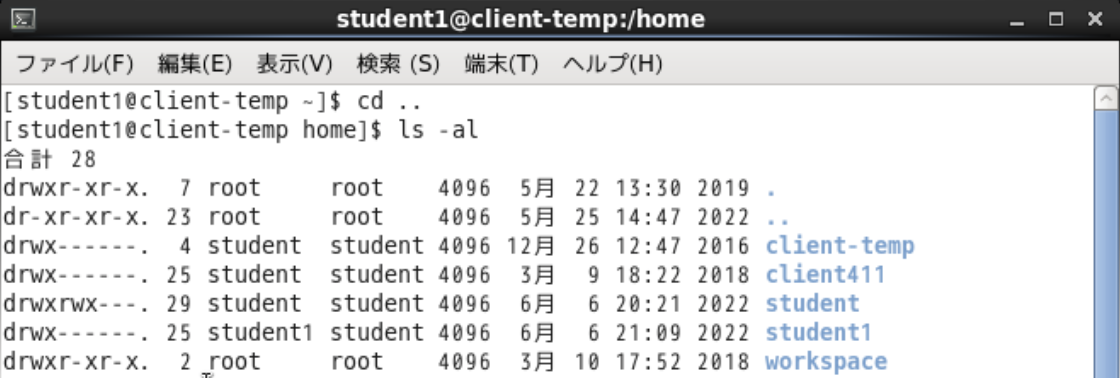
\includegraphics[scale=0.6]{pic12.png}
  \caption{}
\end{figure}

まず、「student」と「student1」は同一のグループ「student」に属して
いることが確認できる、さらに、同一グループのアクセス権限設定が「r(読み込み
)w(書き込み)x(実行)」となっているため、同一グループに属していれば、自由に内容を書き換えたり、
新しくファイルを作ることが可能な状態となっている。以下の図は、student1に
おいて実行されたコマンドのログである。

\begin{figure}[h]
  \centering
  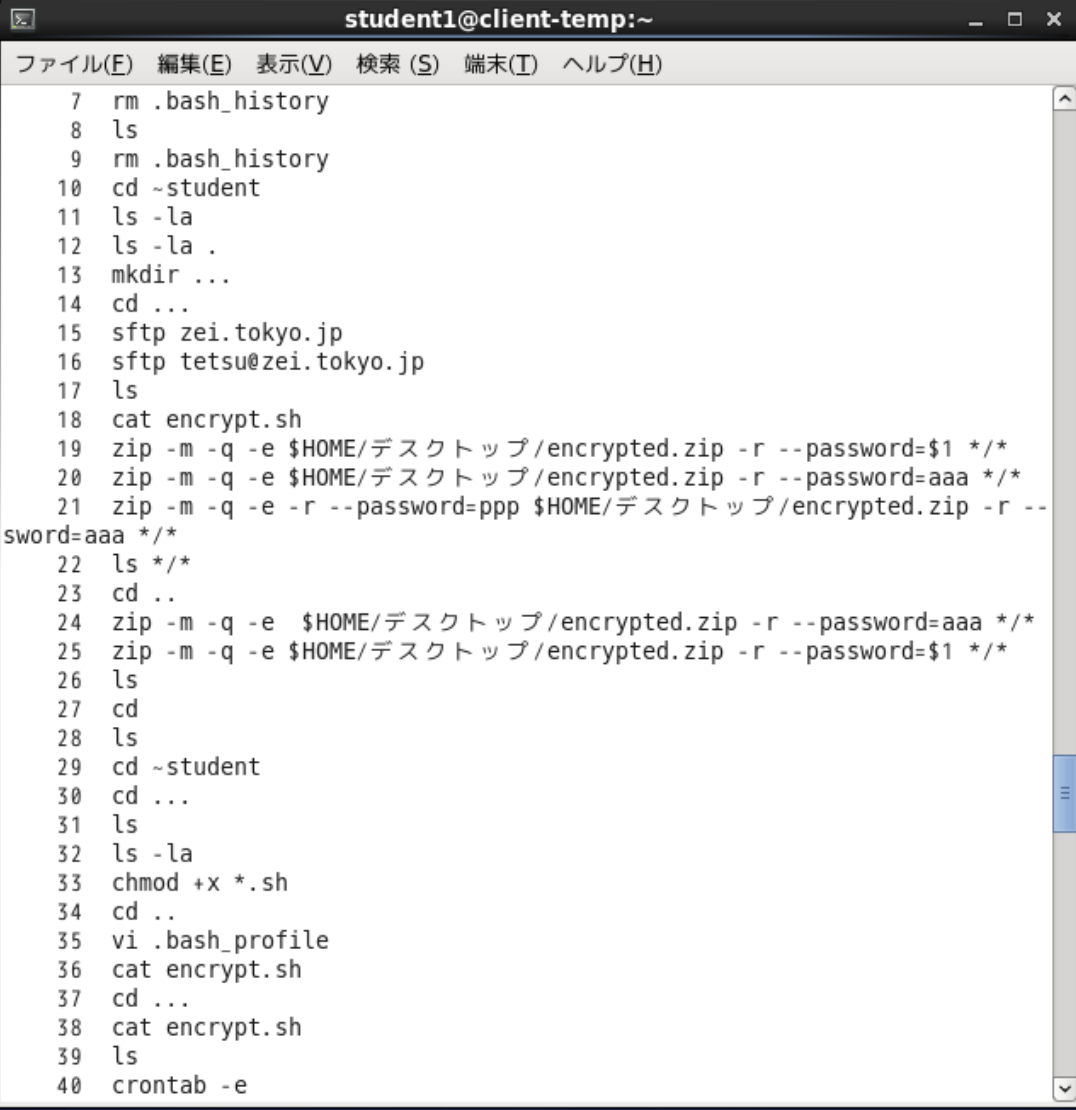
\includegraphics[scale=0.6]{pic13.png}
  \caption{}
\end{figure}

10行目においてstudentのホームディレクトリに移動し、13行目でディレクトリ「...」
を生成、そして、あらかじめサーバ準備しておいた攻撃ファイルを15,16行目でダウンロード
している。また、35行目で「bash\_profile」の内容を変更したことで、次回ユーザ
studentがログインしたときに、全ての攻撃が行われるという流れである。\\
この攻撃に対しての対策方法としては、まずユーザ「student1」にしっかりとパスワード
をかけておくことが挙げられる。また、同一グループに対するアクセス権限を,読み込み
限定などにすることで、新たなファイルの生成や、内容の書き換えを防ぐことが重要である。

\end{document}

